% Vector replica of Fig. 10 of the submitted manuscript (Fig10.jpeg, 1654 x 1083 px); coordinates are the pixel
% positions of the original drawing (x right, y down), text and layout unchanged.
\documentclass[border=2pt]{standalone}
\usepackage[T1]{fontenc}\usepackage[scaled]{helvet}\renewcommand\familydefault{\sfdefault}
\usepackage{tikz}\usetikzlibrary{arrows.meta}
\definecolor{bxc}{RGB}{42,82,98}\definecolor{txc}{RGB}{55,55,55}
\begin{document}
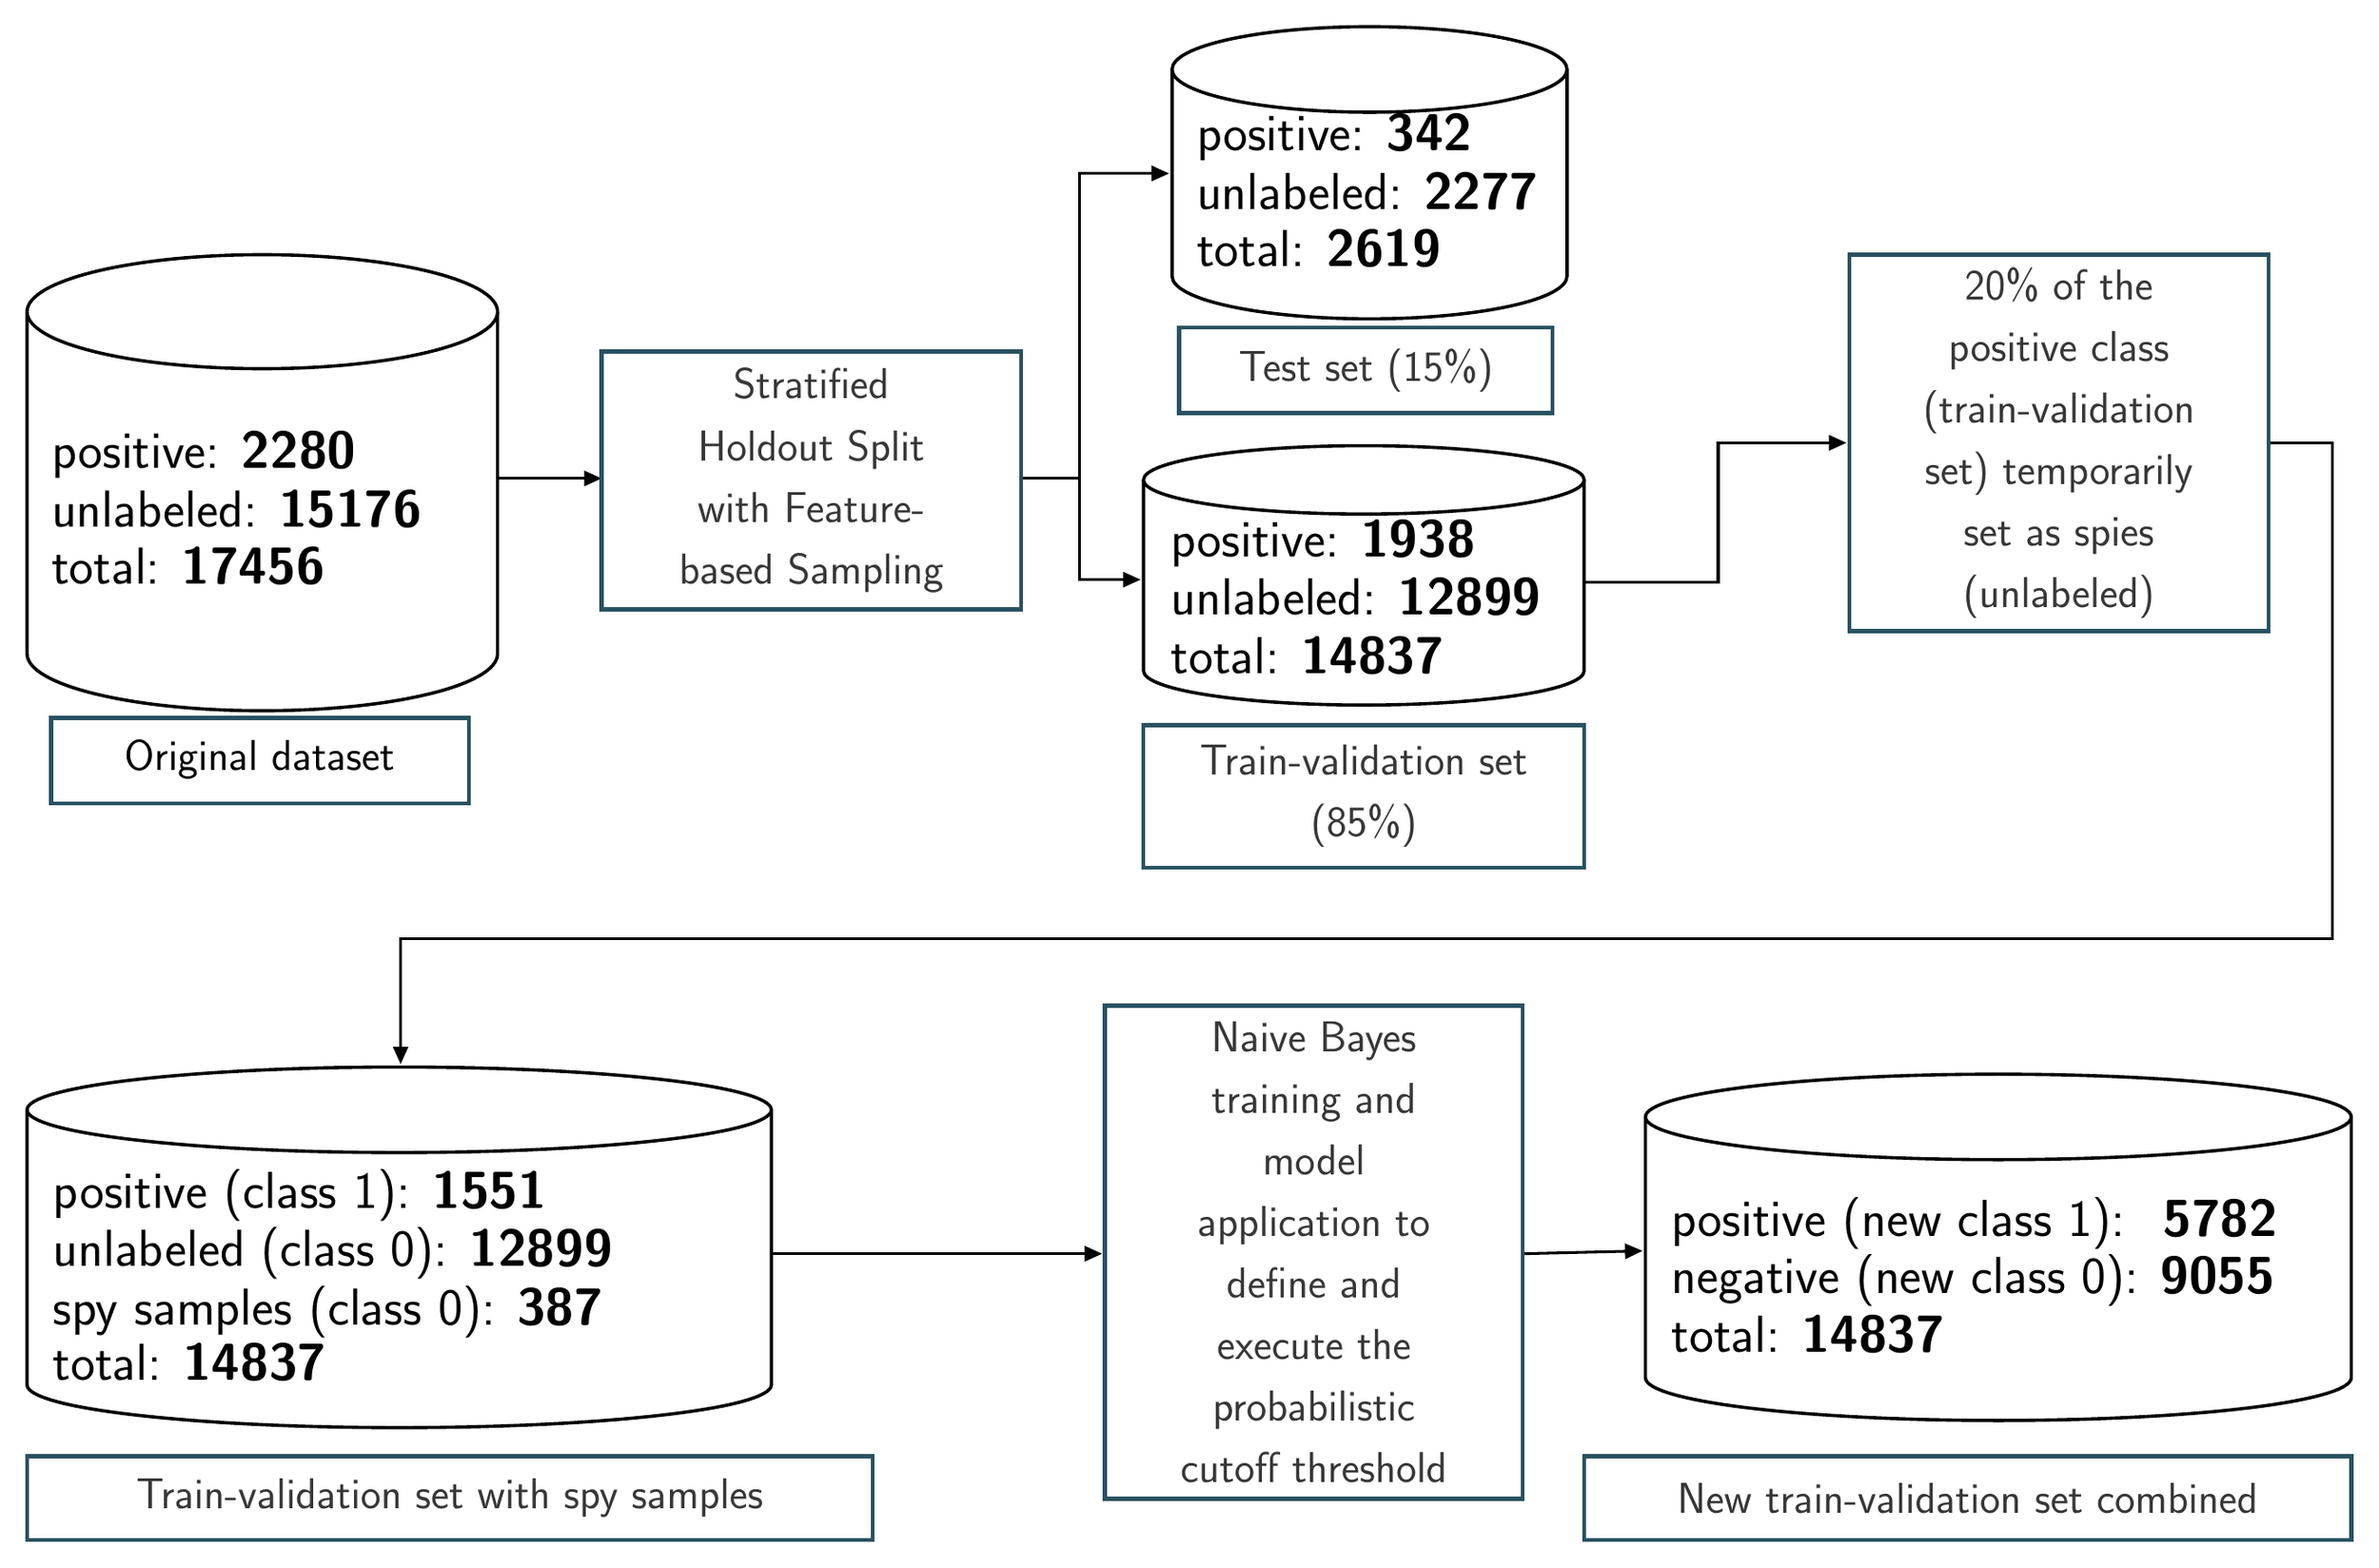
\begin{tikzpicture}[x=0.02cm, y=-0.02cm,
  cl/.style={anchor=base west, font=\fontsize{20}{24}\selectfont, inner sep=0pt},
  bt/.style={align=center, font=\fontsize{19}{24.6}\selectfont, text=txc, inner sep=0pt},
  bx/.style={draw=bxc, line width=1.6pt},
  arr/.style={-{Triangle[length=7pt,width=6pt]}, line width=1.1pt}]
\newcommand\cyl[5]{\fill[white] (#1,#3) -- (#1,#4) arc[start angle=180, end angle=0, x radius={(#2-#1)/2}, y radius=#5] -- (#2,#3) -- cycle;
  \draw[line width=1.3pt] (#1,#3) -- (#1,#4) arc[start angle=180, end angle=0, x radius={(#2-#1)/2}, y radius=#5] -- (#2,#3);
  \draw[line width=1.3pt, fill=white] ({(#1+#2)/2},#3) ellipse[x radius={(#2-#1)/2}, y radius=#5];}
\newcommand\B[5]{\draw[bx] (#1,#2) rectangle (#3,#4); \node[bt] at ({(#1+#3)/2},{(#2+#4)/2}) {#5};}
% arrows
\draw[arr] (340,327) -- (413,327);
\draw[line width=1.1pt] (707,327) -- (748,327); \draw[arr] (748,327) -- (748,113) -- (811,113); \draw[arr] (748,327) -- (748,398) -- (791,398);
\draw[arr] (1102,400) -- (1196,400) -- (1196,302) -- (1286,302);
\draw[arr] (1582,302) -- (1627,302) -- (1627,650) -- (272,650) -- (272,738);
\draw[arr] (532,871) -- (764,871);
\draw[arr] (1059,871) -- (1143,869);
% cylinders
\cyl{10}{340}{210}{450}{40} \cyl{813}{1090}{40}{185}{30} \cyl{793}{1102}{328}{462}{24}
\cyl{10}{532}{770}{963}{30} \cyl{1145}{1640}{775}{958}{30}
\node[cl] at (27,320) {positive: \textbf{2280}}; \node[cl] at (27,361) {unlabeled: \textbf{15176}}; \node[cl] at (27,401) {total: \textbf{17456}};
\node[cl] at (830,97) {positive: \textbf{342}}; \node[cl] at (830,138) {unlabeled: \textbf{2277}}; \node[cl] at (830,178) {total: \textbf{2619}};
\node[cl] at (812,382) {positive: \textbf{1938}}; \node[cl] at (812,423) {unlabeled: \textbf{12899}}; \node[cl] at (812,464) {total: \textbf{14837}};
\node[cl] at (28,839) {positive (class 1): \textbf{1551}}; \node[cl] at (28,880) {unlabeled (class 0): \textbf{12899}};
\node[cl] at (28,921) {spy samples (class 0): \textbf{387}}; \node[cl] at (28,960) {total: \textbf{14837}};
\node[cl] at (1163,859) {positive (new class 1): \ \textbf{5782}}; \node[cl] at (1163,899) {negative (new class 0): \textbf{9055}};
\node[cl] at (1163,940) {total: \textbf{14837}};
% boxes
\draw[bx] (27,495) rectangle (320,555); \node[font=\fontsize{18}{20}\selectfont, text=black] at (173,524) {Original dataset};
\B{413}{238}{707}{419}{Stratified\\Holdout Split\\with Feature-\\based Sampling}
\B{818}{221}{1080}{281}{Test set (15\%)}
\B{793}{500}{1102}{600}{Train-validation set\\(85\%)}
\B{1288}{170}{1582}{434}{20\% of the\\positive class\\(train-validation\\set) temporarily\\set as spies\\(unlabeled)}
\B{766}{697}{1059}{1043}{Naive Bayes\\training and\\model\\application to\\define and\\execute the\\probabilistic\\cutoff threshold}
\B{10}{1013}{603}{1072}{Train-validation set with spy samples}
\B{1102}{1013}{1640}{1072}{New train-validation set combined}
\end{tikzpicture}
\end{document}
